% !TeX root = ../main.tex
% Add the above to each chapter to make compiling the PDF easier in some editors.
\chapter{Performance and Evaluation}\label{chapter:performance}
\section{Deployment}
The proposed Android application and server have been tested on 16 devices for six day from 30.05.2019 until 04.06.2019. However, evaluating the lastSeen timestamp of the users showed that only 13 installations were active after 31.05.2019. The server was deployed\footnote{The version deployed during field testing can be found at https://github.com/SimonVanEndern/location-server/releases/tag/v1.0 The final version provides the same functionality but includes improvements (e.g. bug-fixes, comments, ...) over the deployed version.} in the IBM Cloud as a 128 MB node.js instance. The database was hosted as a free version at mongodb.com.

We ran each of 7 requests on a daily basis and also for each timespan of several days within this period. The results can be found in the following tables\footnote{The results are also available in JSON format at https://github.com/SimonVanEndern/tum-thesis-latex/tree/master/published/results}. The results of aggregation 8 were modified in order to protect user priacy. We used this testing period also to improve the performance of the server as well as the Android application and to find and remove bugs.

\begin{table}[]
	\parbox{.45\linewidth}{
		\centering
		\begin{tabular}{|l|l|l|}
			\hline
			\multicolumn{3}{|c|}{\textbf{Average time spent running}}          \\ \hline
			\textbf{Time period / Day} & \textbf{N} & \textbf{Value {[}min{]}} \\ \hline
			30.09.2019                 & 10         & 1.43                     \\ \hline
			31.05.2019                 & 10         & 1.21                     \\ \hline
			30.05.2019 - 31.05.2019    & 10         & 1.96                     \\ \hline
			30.05.2019 - 31.05.2019    & 10         & 1.89                     \\ \hline
			30.05.2019 - 01.06.2019    & 10         & 1.73                     \\ \hline
			30.05.2019 - 03.06.2019    & 9          & 1.79                     \\ \hline
			03.06.2019                 & 9          & 1.95                     \\ \hline
			04.06.2019                 & 8          & 0                        \\ \hline
			30.05.2019 - 04.06.2019    & 8          & 1.55                     \\ \hline
			01.06.2019 - 04.06.2019    & 7          & 0.99                     \\ \hline
			31.06.2019 - 04.06.2019    & 7          & 0.83                     \\ \hline
			02.06.2019 - 04.06.2019    & 7          & 1.05                     \\ \hline
			03.06.2019 - 04.06.2019    & 7          & 0.16                     \\ \hline
		\end{tabular}
		\label{results-running}
		\caption{Average time spent running}
	}
	\hfill
	\parbox{.45\linewidth}{
		\centering
		\begin{tabular}{|l|l|l|}
			\hline
			\multicolumn{3}{|c|}{\textbf{Average time spent walking}}          \\ \hline
			\textbf{Time period / Day} & \textbf{N} & \textbf{Value {[}min{]}} \\ \hline
			30.09.2019                 & 10         & 17.63                    \\ \hline
			31.05.2019                 & 10         & 97.25                    \\ \hline
			30.05.2019 - 31.05.2019    & 10         & 63.20                    \\ \hline
			30.05.2019 - 31.05.2019    & 10         & 78.41                    \\ \hline
			30.05.2019 - 01.06.2019    & 10         & 75.14                    \\ \hline
			01.06.2019                 & 4          & 72.85                    \\ \hline
			30.05.2019 - 03.06.2019    & 9          & 81.94                    \\ \hline
			03.06.2019                 & 9          & 146.49                   \\ \hline
			04.06.2019                 & 8          & 86.77                    \\ \hline
			30.05.2019 - 04.06.2019    & 8          & 61.86                    \\ \hline
			01.06.2019 - 04.06.2019    & 7          & 57.44                    \\ \hline
			31.06.2019 - 04.06.2019    & 7          & 67.63                    \\ \hline
			02.06.2019 - 04.06.2019    & 7          & 51.75                    \\ \hline
			03.06.2019 - 04.06.2019    & 7          & 64.04                    \\ \hline
		\end{tabular}
		\label{results-walking}
		\caption{Average time spent walking}
	}
\end{table}

\begin{table}[]
	\parbox{.45\linewidth}{
		\centering
		\begin{tabular}{|l|l|l|}
			\hline
			\multicolumn{3}{|c|}{\textbf{Average number of steps per day}}     \\ \hline
			\textbf{Time period / Day} & \textbf{N} & \textbf{Value}           \\ \hline
			30.05.2019                 & 5          & 4331.6                   \\ \hline
			31.05.2019                 & 5          & 3439.8                   \\ \hline
			30.05.2019 - 31.05.2019    & 6          & 3278.7                   \\ \hline
			30.05.2019 - 31.05.2019    & 5          & 4030.2                   \\ \hline
			30.05.2019 - 01.06.2019    & 6          & 4271                     \\ \hline
			01.06.2019                 & 1          & 17                       \\ \hline
			30.05.2019 - 03.06.2019    & 5          & 643959                   \\ \hline
			03.06.2019                 & 3          & 455411.3                 \\ \hline
			04.06.2019                 & 3          & 1123                     \\ \hline
			30.05.2019 - 04.06.2019    & 5          & 3622.6                   \\ \hline
			01.06.2019 - 04.06.2019    & 2          & 2088.5                   \\ \hline
			31.05.2019 - 04.06.2019    & 3          & 4681.3                   \\ \hline
			02.04.2019 - 04.06.2019    & 3          & 326363.3                 \\ \hline
			03.04.2019 - 04.06.2019    & 3          & 455903.7                 \\ \hline
		\end{tabular}
		\label{results-steps}
		\caption{Average number of steps per day}
	}
	\hfill
	\parbox{.45\linewidth}{
		\begin{tabular}{|l|l|l|}
			\hline
			\multicolumn{3}{|c|}{\textbf{Average time spent in a vehicle}}     \\ \hline
			\textbf{Time period / Day} & \textbf{N} & \textbf{Value {[}min{]}} \\ \hline
			30.05.2019                 & 10         & 8.24                     \\ \hline
			31.05.2019                 & 10         & 119.92                   \\ \hline
			30.05.2019 - 31.05.2019    & 10         & 68.40                    \\ \hline
			30.05.2019 - 31.05.2019    & 10         & 90.49                    \\ \hline
			30.05.2019 - 01.06.2019    & 10         & 82.19                    \\ \hline
			01.06.2019                 & 4          & 90.40                    \\ \hline
			30.05.2019 - 03.06.2019    & 9          & 62.16                    \\ \hline
			03.06.2019                 & 9          & 71.74                    \\ \hline
			04.06.2019                 & 8          & 35.51                    \\ \hline
			30.05.2019 - 04.06.2019    & 8          & 59.34                    \\ \hline
			01.06.2019 - 04.06.2019    & 7          & 51.07                    \\ \hline
			31.05.2019 - 04.06.2019    & 7          & 68.20                    \\ \hline
			02.04.2019 - 04.06.2019    & 7          & 48.89                    \\ \hline
			03.04.2019 - 04.06.2019    & 7          & 45.96                    \\ \hline
		\end{tabular}
		\label{results-vehicle}
		\caption{Average time spent in a vehicle}
	}
\end{table}

\begin{table}[]
	\centering
	\begin{tabular}{|l|l|l|}
		\hline
		\multicolumn{3}{|c|}{\textbf{Average time spent biking}}           \\ \hline
		\textbf{Time period / Day} & \textbf{N} & \textbf{Value {[}min{]}} \\ \hline
		30.05.2019                 & 10         & 2.29                     \\ \hline
		30.05.2019 - 31.05.2019    & 10         & 11.10                    \\ \hline
		01.06.2019                 & 4          & 14.99                    \\ \hline
		03.06.2019                 & 9          & 31.03                    \\ \hline
		04.06.2019                 & 8          & 23.81                    \\ \hline
	\end{tabular}
	\label{results-biking}
	\caption{Average time spent biking}
\end{table}

\begin{table}[]
	\centering
	\begin{tabular}{|l|l|l|}
		\hline
		\multicolumn{3}{|c|}{\textbf{Listing of average number of steps per day per of each participant}} \\ \hline
		\textbf{Time period / Day}         & \textbf{N}        & \textbf{Values}                          \\ \hline
		30.05.2019                         & 10                & 1661, 1246, 3195, 7714, 7842             \\ \hline
		31.05.2019                         & 10                & 2747, 775, 3924, 9203                    \\ \hline
		30.05.2019 - 31.05.2019            & 10                & 550, 2905, 3195, 775, 88828, 3419        \\ \hline
		30.05.2019 - 31.05.2019            & 10                & 550, 8828, 5145, 3195, 2433              \\ \hline
		30.05.2019 - 01.06.2019            & 10                & 8126, 3195, 283, 8828, 1629, 3565        \\ \hline
		01.06.2019                         & 4                 & 17                                       \\ \hline
		30.05.2019 - 03.06.2019            & 9                 & 598, 3195, 1669, 8828, 3205505           \\ \hline
		03.06.2019                         & 9                 & 914, 1042, 1364278                       \\ \hline
		04.06.2019                         & 8                 & 1103, 13332, 934                         \\ \hline
		30.05.2019 - 04.06.2019            & 8                 & 757, 1719, 8828, 3614, 3195              \\ \hline
		01.06.2019 - 04.06.2019            & 7                 & 826, 33511                               \\ \hline
		31.05.2019 - 04.06.2019            & 7                 & 757, 9203,, 4084                         \\ \hline
		02.04.2019 - 04.06.2019            & 7                 & 974691, 1231, 3168                       \\ \hline
		03.04.2019 - 04.06.2019            & 7                 & 1364278, 1231, 2202                      \\ \hline
	\end{tabular}
	\label{results-steps-listing}
	\caption{Average number of steps per day of each user}
\end{table}

\section{Data Consumption}
The application used very few data. We are happy that some research participants provided us information about the app's data usage. Table XX shows the collected results of this rather qualitative analysis. Screenshots are attached in the appendix. On most phones the data consumption for 6 days was below 20 MB. The highest data consumption was 376 and is attributable to an error that occurred on the last day of the testing period. Requests were sent multiple up to unlimited times. This explains the high data consumption reported also by two other participants. This error was present during the whole testing period but interacted with another error that occurred only on the last day. This suggests, that the actual data consumption of the application would be far lower in practise (with the errors being fixed).
Also the few available reports about battery consumption indicate a rather moderate battery consumption.

\section{Results}
We computed the aggregated results for each of the 6 days of the testing period separately and for 5 timespans from each of those days until the last day. The results can be seen in figure XXX. 
On most of the days the average time spent walking is roughly around one hour per day. Nevertheless, on the 3rd of June the value is clearly higher and 31st as well. We do not see any reason for this spike -- 03.06. is a regular work day - nevertheless, the value is not that high as it would suggest errors. The value on the first day being below the other values is definitely attributable to the fact that we started to roll out the application on this day.
The average time running is around 1-2 minutes per day. This is not surprising. The only scenarios usually are when somebody has to catch some transport or actively is running (and might probably not carry his or her phone).
Due to an error in the setup, we only have the daily average data for the time spent biking which ranges from 11 to 31 minutes per day and sounds realistic regarding that the participants where all in Munich.
The time spent in a  vicle ranges from half an hour to 90 minutes on average per day and has one spike of almost 2 hours on 31.06. This can be explained as one of our research team had a very long car ride on this day. Comparing the data with the registered trajectories, there is another pretty long car ride which might have attributed to the high average of 90 minutes per day. 
The average steps per day range in the lower range of some thousands. Though, there are some values which clearly expose an error in our aggregation process. Excluding these definitely incorrect values from the statistics, the values all are in an expected range. 
Investigating the list of average steps, it is clear that the erro did not occur in the aggregation process but in the process of local aggregation of data. There is always maximum one value off, all other values are withinn an expected range. The zero values are due to non step sensor being present on the respective phones (which are excluded in the average aggregation).
Using the algorithm described in chapter \ref{local-data-aggregation} a total of 406 trajectories where computed out of the raw GPS data. A part of the trajectories are shown in figure \ref{trajectories1} and \ref{trajectories2}. The complete results can be found in the appendix. \footnote{Whenever the trajectory started or ended clearly in a precise private location e.g. housing, we modified this location. So the results actually do not represent real trajectories anymore}

\begin{figure}[h!]
	\caption{Trajectories}
	\label{trajectories1}
	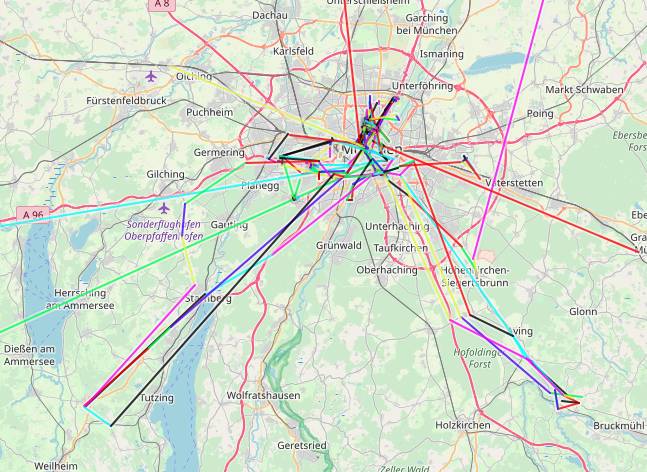
\includegraphics[width=\textwidth]{data/trajectories-2.png}
\end{figure}

\begin{figure}[h!]
	\caption{Trajectories}
	\label{trajectories2}
	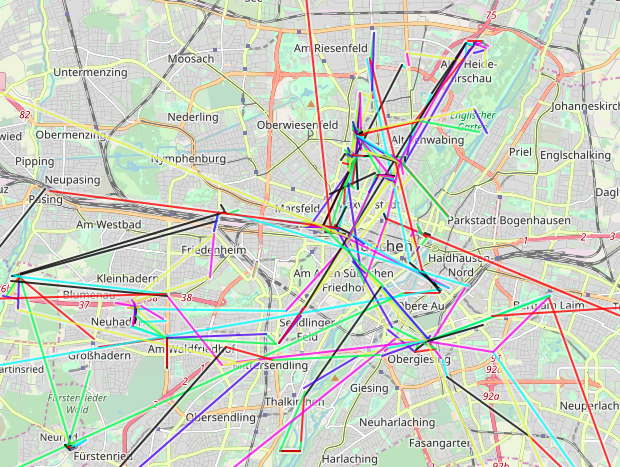
\includegraphics[width=\textwidth]{data/trajectories-3.png}
\end{figure}

\section{Implications}
Our results show clearly, that there is no privacy risk imposed on the user upon publication of the aggregated average data. Especially it was shown that when repeating the request, the user base changes and the value accordingly. So, publishing pure mean values of analysis does not impose any privacy risk to the user. Furthermore we showed exemplary with the steps aggregation, that also the collection of the users' average values is possible without posing a privacy risk to the user. This implies, that not only the aggregation of mean values but also the collection of locally aggregated data is possible without privacy concerns. We do not see any possibility to infer that the same user took part in different aggregations. There might be a chance in case of a very high steps value and a very high mean time spent walking or running, but this would only allow to assume the same user being present in both aggregations which allows for no further inference.

Nevetheless when collecting the average data, through overlapping requests e.g. one from 30.05 - 02.06 and one from 01.06. - 04.06 it might be possible to infer the exact date of some of the data present in both requests. Though, we do not see any risk aggregating on a daily basis or even hourly if there is any reason for this granularity level. Thus, the inference does no harm.

In more than 90\% of cases, local trajectories could match an activity for more than 90\% of the time.
The experimental collection of trajectories clearly shows privacy risks as pointed out in XX. Nevertheless, the data suggests that those trajectories can easily be linked locally and identify changing of transport system or e.g. metro line. For example at the locations Giselastraße, Odeonsplatz and central station and other locations, many trajectories end respectively start. Mapping the current activity to those trajectories enables aggregations as mentioned in chapter \ref{aggregation-schemes}. Noting that locally all data points of the trajectories are available, it is also easy to compute the distance travelled. Also it is possible to compute how many people combine e.g. bike and car or public transport and furthermore identify, which station is most likely (in case of public transport) to be combined with bike.


Also it would be possible to create a "travelled road" or "travelled public transport" map by aggregating the trajectories data so that there would not be multiple trajectories but each road either marked used or not used. This way it would be possible to identify that a user lives in a certain area but could not link to the work location due to obfuscation with other routes joining. This map would on the other hand allow to have a feeling of which areas are covered by the data / app. This map could also be extended with the average speed on the respective road depending on vehicle or bike and also compare whether bike is faster.

Computing time to work and average time at work.

It also allows for computing how many people go by car, bike, or mixed to work.

We also started an aggregation a second time - walking from 30.05 - 01.06. which shows as expected a different result than the original aggregation due to the 10 users being not the same users as in the first request. Nevertheless, the value is not far off as expected.

TODO:
The trajectories also show, that in the not anonymized data set we had at hands, often trajectories of which the endpoints did not clearly indicate an ongoing, the numeration of the trajectory indicated that they were connected. This 1. highlights the importance of list order randomization and 2. shows that our algorithm of finding trajectories still has possibilities for improvement. (TODO: Randomize order in published data set)

\section{Scenario Traffic Jam}
A typical scenario of google maps is o notify users about traffic jams and suggest alternate routes. The calculation of alternate routes taking traffic jams into account can clearly happen locally with the maps data. Google maps works when offline. The data about all current traffic jams can also be made publicly available through a server. Generating the data can also happen without exposing raw data: The user downloads a map containing data of the usual speeds at each street. While the user is driving, the app registers the speed and compares it in the background to the normal speed. If the speed is significantly lower, the user chooses a random list of known users and sends the signal as a request for those users to the server. They randomly according to a fixed percentage choose to inform the server about the traffic jam or forward the signal another time. The signal contains a unique id thus that the server even when receiving it muliply times knows it is from one user. If more than a threshold of signals is received, a traffic jam is "created". Also the request is not forwarded anymore after a certain time to stop it from spreading unlimited.

